\documentclass[11pt,a4paper]{report}

% Packages
\usepackage{graphicx}
\usepackage{amsmath}
\usepackage{hyperref}
\usepackage{setspace}
\usepackage{listings}
\usepackage{xcolor}  % Include xcolor for text color
\usepackage{abstract}
\usepackage{float}


% Title and Author (adjust the spacing as needed)
\title{\LARGE \textbf{Assignment ADIPCV 2025}}
\author{Mouzakitis Nikolaos}
\date{\large On: \today}

% Begin Document
\begin{document}

% Title Page
\makeatletter
\begin{titlepage}
    \centering
    \vspace*{1cm}
       { 
\includegraphics[width=6cm]{ELMEPA.png}}\\[1cm]

    {\LARGE \textbf{Glioma-meningioma tumor classification on MRI scans }}\\[1cm]
    
    
    \textbf{Written By:}{Nikolaos Mouzakitis}\\[1cm]
    \date{\large Date Last Edited: \today}
    {\@date\\}
\end{titlepage}
\makeatother
% Abstract
\chapter*{Abstract}
\addcontentsline{toc}{chapter}{Abstract}
This report presents an automated system 
for classifying brain tumors as either meningioma or glioma 
using MRI images. 
In the followed approach radiomic features from PyRadiomics with custom-designed intensity,
shape, symmetry, and frequency domain features are blended together in order to 
train machine learning models for classification purposes. 
Two classifiers, Random Forest and Multi-Layer Perceptron (MLP) Neural Network) are evaluated. 
Feature extraction was performed using SimpleITK for image loading, 
OpenCV for preprocessing, and scikit-learn for modeling. 
Results showed that both models achieved good performance, 
with Random Forest outperforming the neural network slightly in terms of 
accuracy and AUC, demonstrating
the feasibility of using hybrid feature 
engineering for medical image classification.

% Table of Contents
\tableofcontents

% Chapters
\chapter{Introduction}
Brain tumors are among the most complex and dangerous 
diseases affecting the central nervous system. 
Early and accurate diagnosis is crucial in order to achieve effective treatment on time. 
Magnetic Resonance Imaging (MRI) is a widely used modality for detecting 
and characterizing brain tumors due to its high resolution and contrast.

Meningiomas and gliomas are two of the common types of primary brain tumors with 
different prognoses and treatment strategies. 
Manual differentiation by radiologists can be time-consuming 
and subject to variability. 
One solution for supporting clinical decision making, is an automated classification system.
A system like this, can reduce diagnostic workload, 
increase consistency, and potentially improve early detection rates. 
It also provides a framework for future research 
into AI-assisted diagnostics in radiology or related application domains.

In this project, a machine learning-based system that automatically 
classifies MRI images into meningioma or glioma categories 
using custom handcrafted, frequency and radiomic features 
is developed and evaluated.

\chapter{Related Work}

\chapter{Methodology-Implementation}
    \section{Hw and Sw Requirements}
	\par The software stack used to implement the classification system consists of Python libraries
	such as \textit{SimpleITK, OpenCV, scikit-learn, PyRadiomics, matplotlib, seaborn}.
    \section{Data Details}
	MRI images were sourced from \cite{data}, which contains 7023 MRI images of human brain, divided 
	in 4 categories: \textit{glioma - meningioma - no tumor and pituitary}.
	For this report's purpose the first two categories are utilized, and selected 1000 MRI images from both \textit{glioma} and
	\textit{meningioma} classes.

    \section{Method}
	
	\par Related to the methodology of the classification system, for the preprocessing step
	all images are loaded using SimpleITK
	and converted into NumPy arrays and their respective pixel intensities are 
	normalized into the range of grayscale images ([0, 255]).
	In the next step a 4 pixel masking takes place, in order to reduce the black surrounding areas
	appearing in every MRI image. This border mask is applied and excludes irrelevant regions at the 
	edges of the images. The number of the extracted features can be divided into three subcategories:

	1)\textit{Features acquired from Pyradiomics(}: by utilization of PyRadiomics first-order statistics (mean, variance, entropy) and
	texture features (GLCM, GLRLM, GLSZM) are extracted.
	\newline
	2)\textit{Custom Features}: have been designed and implemented in order to intuitively help detecting a tumor alike
	object on an MRI image. (\textit{intensity\_skewness, intensity\_outlier\_score, high\_intensity\_area, max\_circularity,
	top3\_circularity\_mean, solidity\_outlier, abnormal\_area\_ratio, circular\_area\_score, asymmetry\_score, asymmetry\_outlier,
	boundary\_sharpness\_mean, boundary\_sharpness\_max, boundary\_sharpness\_outlier}.

	3)\textit{Frequency Domain Features}: Energy, entropy, mean, and skewness in low, mid, and high-frequency 
	bands using FFT.
	

	By conducting the feature extraction process, \textit{min-max} normalization is performed in all the generated feature values
	mapping them on the [0, 1] range. 
		\begin{figure}[h]
			\centering
			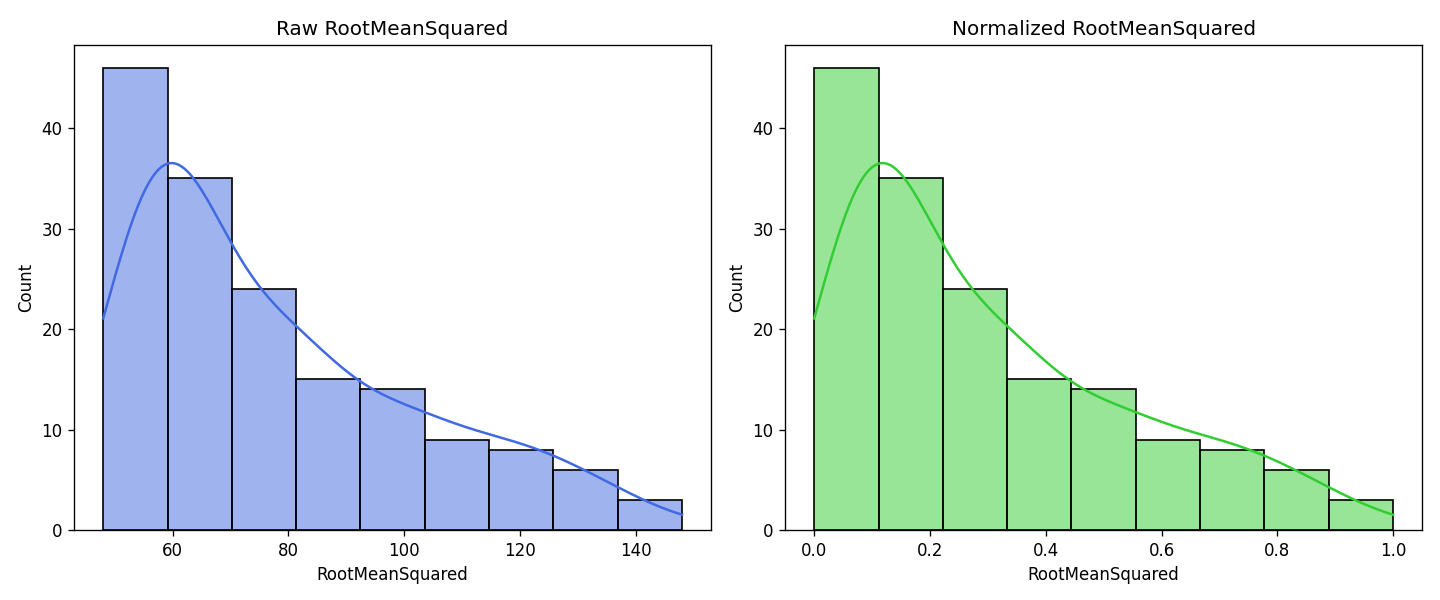
\includegraphics[width=1.1\textwidth]{images/RootMeanSquared.png}
			\caption{Comparisson of feature distribution prior and after the \textit{min-max} normalization.}
			\label{fig1:}
		\end{figure}		



    \section{Evaluation Measures}
		
		\par In the classification stage, two different classifiers have been trained and evaluated, a Random Forest classifier
		and a MultiLayer Perceptron Neural Network.

	\subsection{Classification with texture, shape and statistical features}
	
		\begin{figure}[h]
			\centering
			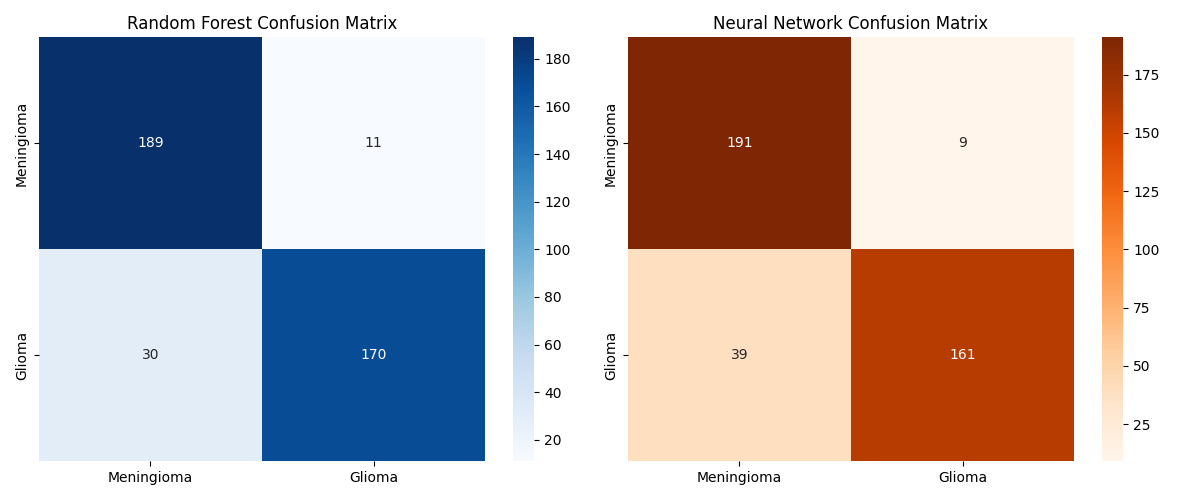
\includegraphics[width=1.1\textwidth]{images/classification_pyradiomics.png}
			\caption{Metric results.}
			\label{fig1:}
		\end{figure}		

		\begin{figure}[h]
			\centering
			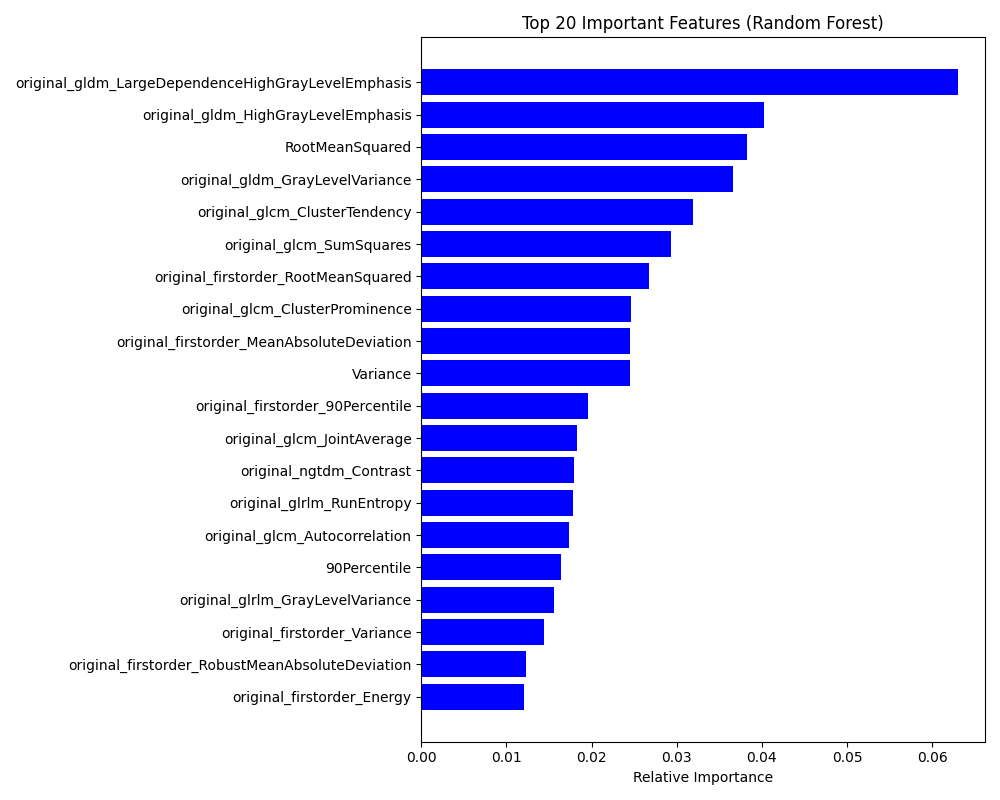
\includegraphics[width=0.9\textwidth]{images/top20_rf_pyradiomics.png}
			\caption{Top20 features of RF.}
			\label{fig1:}
		\end{figure}		

		\begin{figure}[H]
			\centering
			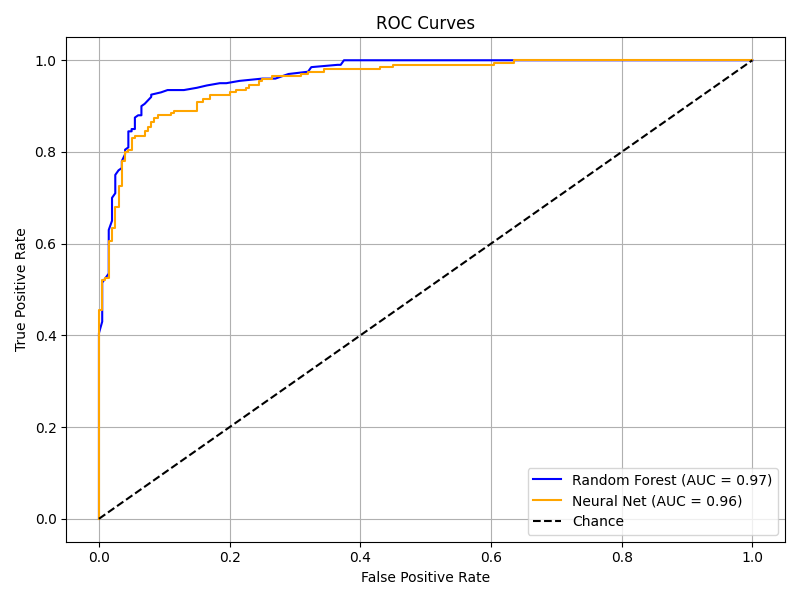
\includegraphics[width=0.9\textwidth]{images/roc_pyradiomics.png}
			\caption{RoC curves for RF and MLP-nn.}
			\label{fig1:}
		\end{figure}		

		\begin{figure}[H]
			\centering
			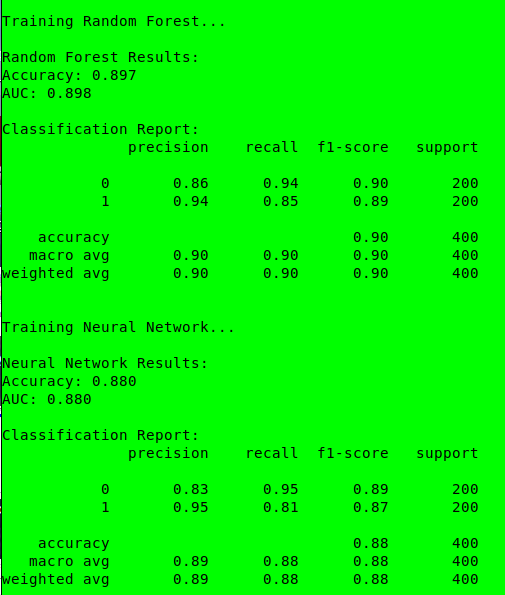
\includegraphics[width=0.5\textwidth]{images/report_pyradiomics.png}
			\caption{Classification report}
			\label{fig1:}
		\end{figure}		

	\subsection{Classification with frequency features}
		\begin{figure}[h]
			\centering
			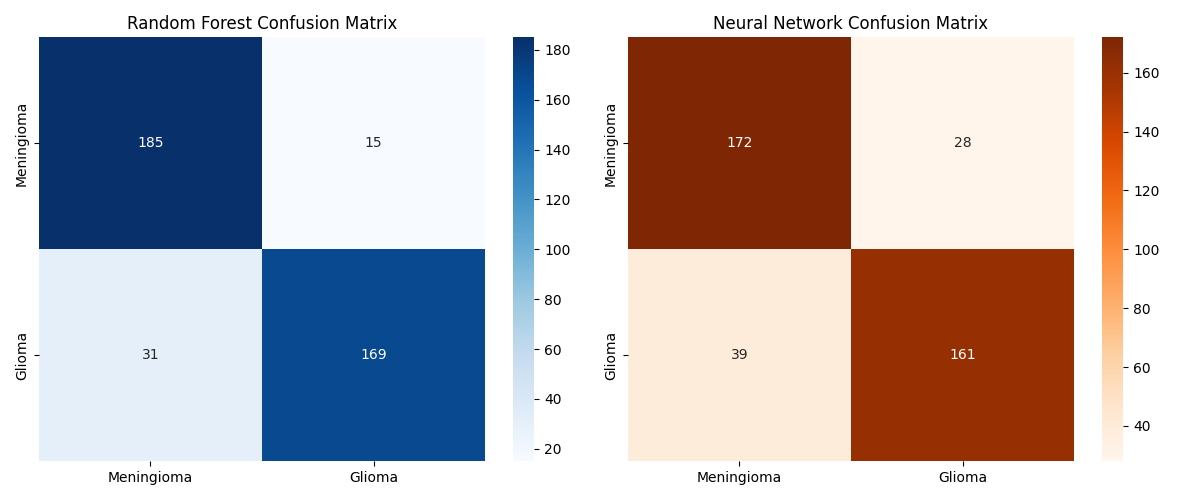
\includegraphics[width=1.1\textwidth]{images/freq_metrics.png}
			\caption{Metric results.}
			\label{fig1:}
		\end{figure}		

		\begin{figure}[h]
			\centering
			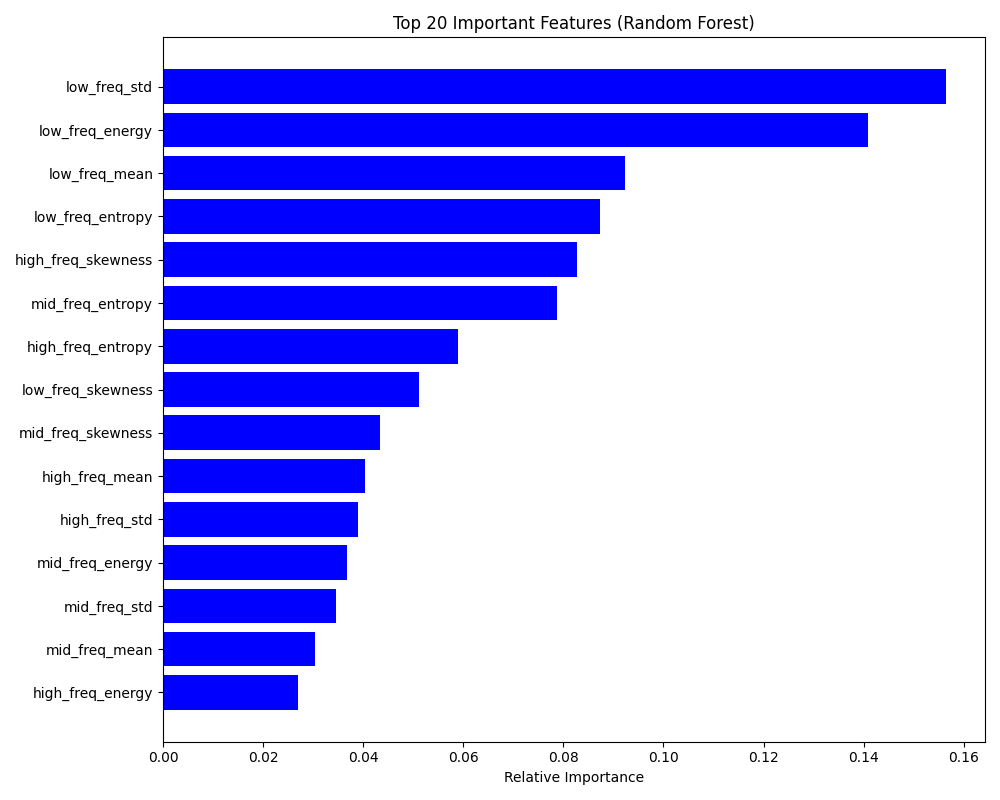
\includegraphics[width=0.9\textwidth]{images/freq_top_rf.png}
			\caption{Top20 features of RF.}
			\label{fig1:}
		\end{figure}		

		\begin{figure}[H]
			\centering
			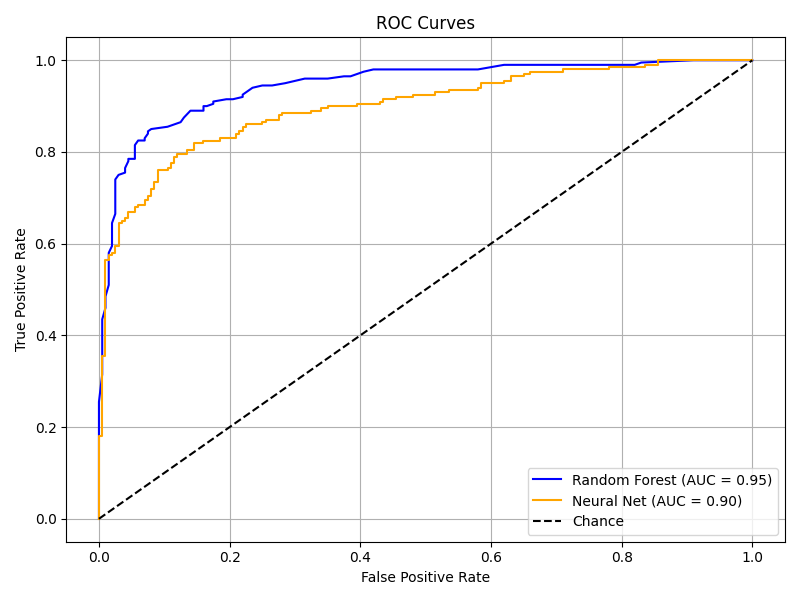
\includegraphics[width=0.9\textwidth]{images/freq_roc.png}
			\caption{RoC curves for RF and MLP-nn.}
			\label{fig1:}
		\end{figure}		

		\begin{figure}[H]
			\centering
			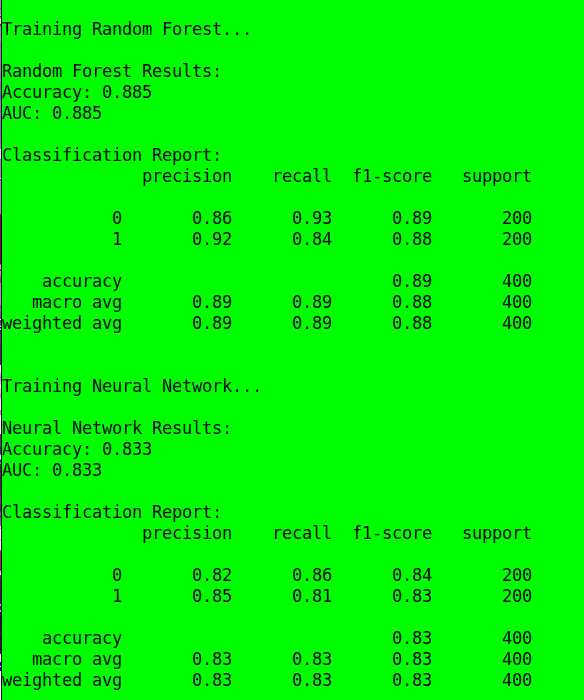
\includegraphics[width=0.5\textwidth]{images/report_freq.png}
			\caption{Classification report}
			\label{fig1:}
		\end{figure}		


	\subsection{Classification utilizing all features}
		\begin{figure}[H]
			\centering
			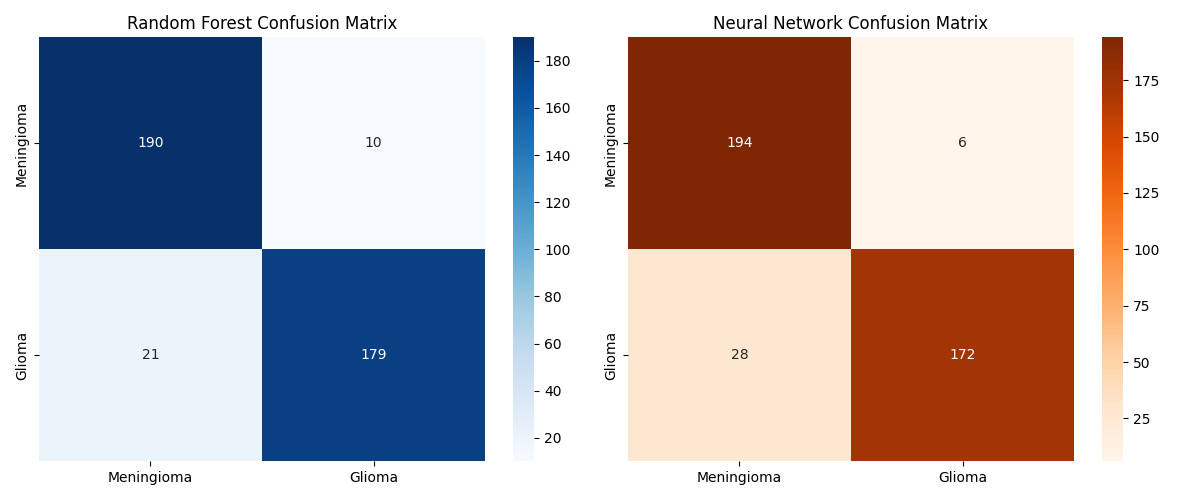
\includegraphics[width=1.1\textwidth]{images/Metrics_all_features.png}
			\caption{Metric results.}
			\label{fig1:}
		\end{figure}		

		\begin{figure}[H]
			\centering
			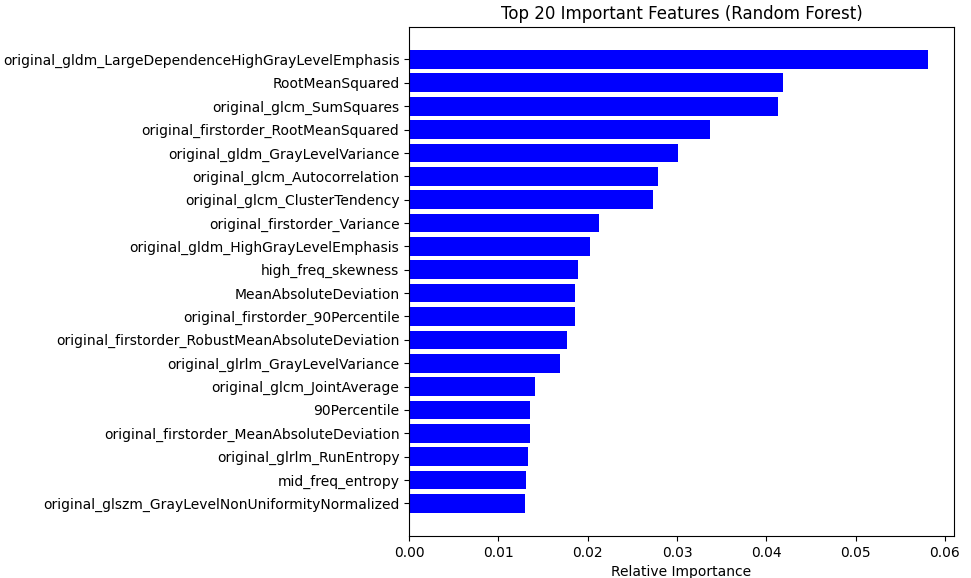
\includegraphics[width=0.9\textwidth]{images/top20features_all_features_rf.png}
			\caption{Top20 features of RF.}
			\label{fig1:}
		\end{figure}		

		\begin{figure}[H]
			\centering
			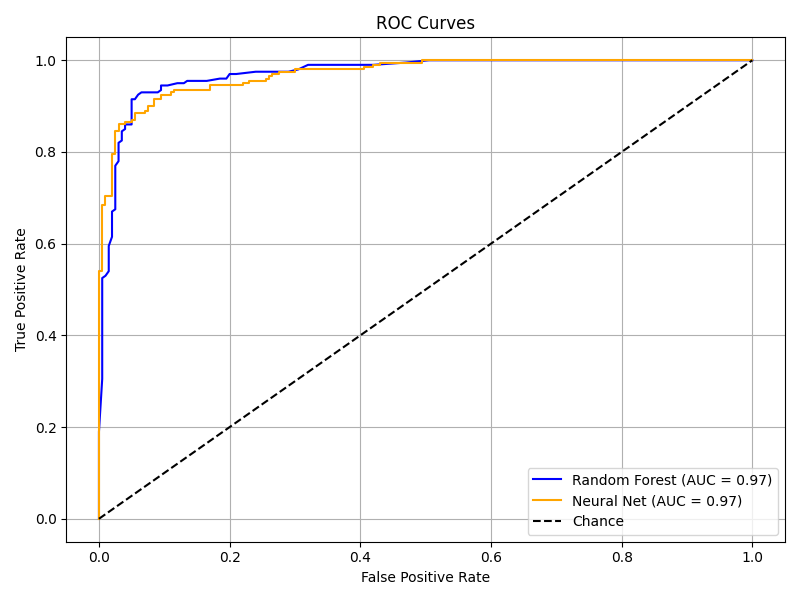
\includegraphics[width=0.9\textwidth]{images/roc_curves_all_features.png}
			\caption{RoC curves for RF and MLP-nn.}
			\label{fig1:}
		\end{figure}		

		\begin{figure}[H]
			\centering
			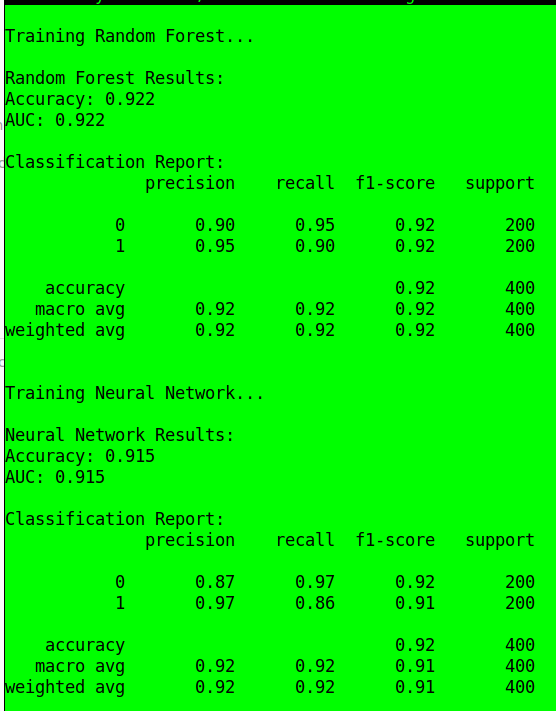
\includegraphics[width=0.5\textwidth]{images/report_all_features.png}
			\caption{Classification report}
			\label{fig1:}
		\end{figure}		


	

\chapter{Conclusion}

\bibliographystyle{plain}
\bibliography{references}
 
\end{document}
